% ---------------------------------------------------------------------------- %
\section{Conclusions}
\label{ch:conclusions}
% ---------------------------------------------------------------------------- %
The idea of building a Linguometer comes from the need to record the largest
amount of features useful to characterize speech from the motoric point of view.
Although the Linguometer by itself does not have a role in determining
whatsoever speech and manipulation are tightly linked processes, the recorded 
data could be used by the CONTACT Project to verify the claim that a motoric
invariance exist between different speakers.

Building a Linguometer-like setup means integrating recording instrumentation
not suited, or at least not designed, to work with in conjunction with 
other devices.
Furthermore, the CONTACT Project is interested in the simultaneous acquisition
of the motoric gestures of speech.
In this particular context, no Linguometer exists without a proper alignment and
processing of the recorded data.
Moreover, no Linguometer or proper alignment procedure exists without the 
procedures described in Chapter~\ref{ch:linguometer:architecture}, referred 
as the ``Linguometer workflow diagram''.
Although recording simultaneously using the articulograph and the ultrasound
system required to design and build an ad-hoc transducer stand, the Linguometer 
has been integrated by interconnecting the different instrumentation using
standard consumer devices, such as the audio mixer and the audio/video
acquisition card.
Furthermore, the software relies on Open-Source libraries,
programs and languages, although Matlab by Mathworks has been used due its large
consensus in the research field.
The
Linguometer, apart being a fairly complicated setup, is a fairly accessible
method of integrating devices in the field of language and speech research.\\
The final alignment methods presented while describing the \emph{LMTools2}
toolkit are flexible and, eventually, aligning the data recorded via additional
devices  is trivial.
In other words, the Linguometer should be considered both as an experimental
setup for the CONTACT Project and a method for acquiring data streams from 
several different sources.

The goal of the work done for the CONTACT Project was to acquire simultaneously
the largest set of phono-articulatory parameters suitable to investigate the
motoric foundations of speech.
In Chapter~\ref{ch:results} some examples of the 
acquired data were presented, showing
 the methods that brought to the alignment of the 
complete dataset, and the difficulties faced.
Two are the main causes of fault during the recordings: damages of cables and 
software instability.
The first problem could have been easily avoided by simply changing the cables
more often. 
In fact, just before each experiment, one experimenter\footnote{Dr. Marisa
Ferro} prepared the sensors while the author\footnote{Michele Tavella} 
carried out testing procedures
(Chapter~\ref{ch:experiments}).
An accurate and automated analysis of the segmentation and synchronization 
signals was performed by \emph{LMTools1}.
Unfortunately, the cables ruined in the middle of an experiment, and for this
reason it was not possible to recover from the fail.

% ---------------------------------------------------------------------------- %
\begin{figure}
  \centering
	\subfigure[\label{fig:conclusions:end:1}]
	{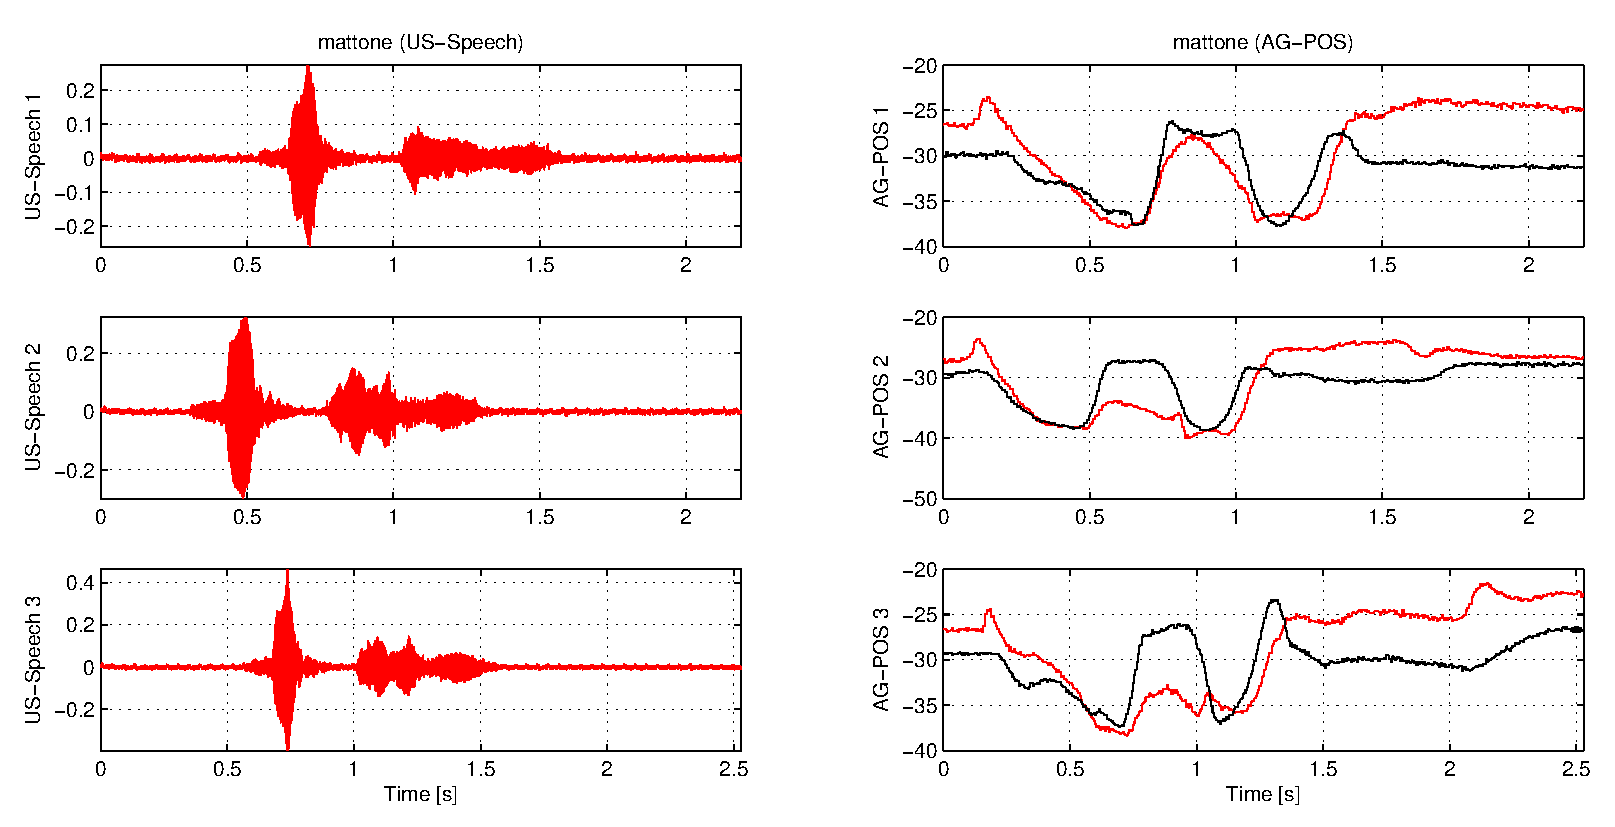
\includegraphics[width=\textwidth]{include/conclusions/images/end_same.eps}}
	
	\subfigure[\label{fig:conclusions:end:2}]
	{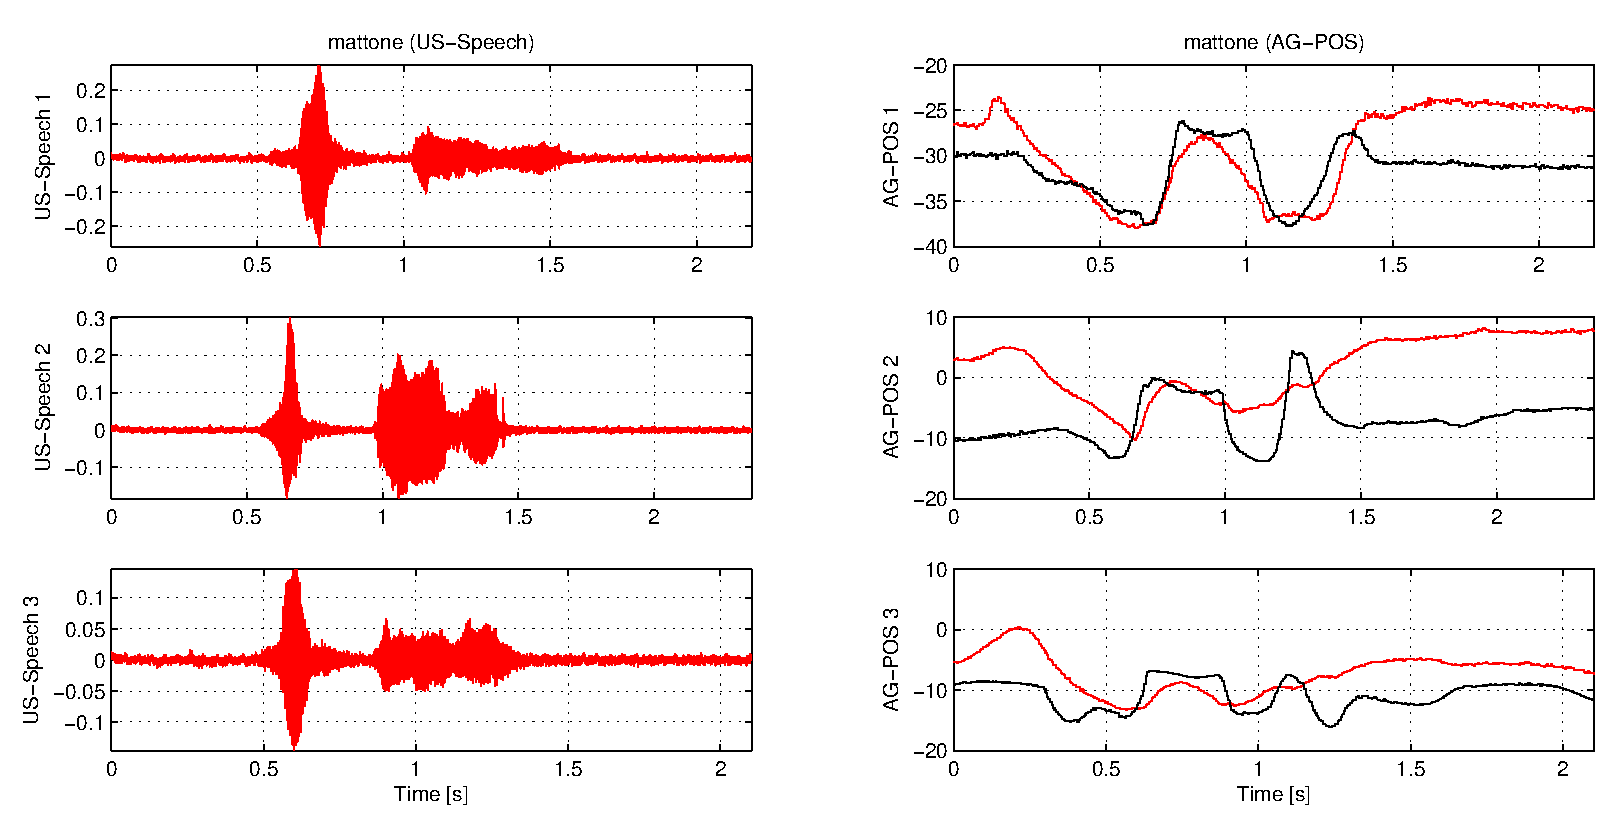
\includegraphics[width=\textwidth]{include/conclusions/images/end_diff.eps}}

	\caption[Speech signals and tongue vertical displacement]
	{\textbf{Speech signals and tongue vertical displacement}: (a) a subject
	(Subject 1) pronounces /mattone/ for three times. 
	(b) Three different subjects (Subjects 1, 4 and 5) pronounce /mattone/.
	For both panels: on the left, waveforms; on the right, vertical
	displacement (Z coordinate) of Sensor 3 (tongue tip, in red) and Sensor 1
	(tongue root, in black).
	The reader may be interested in looking at Figure~\ref{fig:experiments:map}
	and Table~\ref{tab:experiments:subjects} to obtain more details about 
	the positions of the sensors and subjects' age and gender.}
	\label{fig:conclusions:end}
\end{figure}
% ---------------------------------------------------------------------------- %

The problems related to software instabilities that affect the articulograph 
AG500  can not be neglected, specially if the device is designed and 
commercialized to record from human subjects\footnote{It is important to
underline that Carstens Medizinelektronik GmbH is working onto a new version of
the control software that was unfortunately unavailable by the time the
experiments took place.}.
In this particular context, it results clear that over-stressing the subjects
has to be avoided in order not to compromise the both the recordings and the
production of speech.
The vast majority of crashes required to reboot both the control computer and
the articulograph itself. 
It turns out clear that this procedures elongate the duration of an experiment,
thus stressing the subjects.
It is important to specify that the experiments have never been suspended, also
in the cases where the articulograph resulted to be unusable.
Although in those cases the recorded data is far away from being complete, 
part of it could be used for other purposes (e.g.: the speech signals may turn
out to be useful to test the Bayesian model).

\comment{
Besides designing a speech recognizer that relies onto the motoric
representation of speech, the CONTACT Project aims to investigate the motoric
invariance that may characterize the production of speech gestures.
According to Liberman's theoretical framework,
the real constituents of speech are not sounds, but the articulatory gestures 
underlining it.
From this relatively novel point of view, the sender and the receiver of a
message must share a common motor vocabulary, otherwise communication does not
occur~\citep{liberman.mattingly:1985}.
Under the here presented circumstances, speech perception 
depends onto the articulatory gestures that generate the sounds of language.
In other words, the receiver perceives the message sent by the speaker when the
it activates his/her own articulatory gestures.
\citet{fadiga.craighero.etal:2002} demonstrated that speech listening
specifically activates the listener tongue muscles when the presented words
involve important tongue mobilization~(Section~\ref{sec:speech:mirror}).
From a broader perspective, what said provides the background for designing the
Bayesian speech recognizer based on the audio-motor map 
(Chapter~\ref{ch:linguometer}).}

Although the goal of this thesis is not to verify if the motoric configurations
of the articulators are characterized by low variability during speech 
production, a final consideration is done before the end of this dissertation.
Figure~\ref{fig:conclusions:end} shows the waveforms and the vertical
displacement of two sensors glued onto the dorsum of the tongue in two cases.
In the first case, shown in Figure~\ref{fig:conclusions:end:1}, the same subject
pronounces /mattone/ (English: /brick/) for three times.
In the second case, three subjects pronounce /mattone/.
It is clear, by simply looking at the trajectories, that in the first case the
tongue performs similar movements during the three repetitions.
In the case of different subjects, the vertical displacement profiles still look
similar, although the similarities are not comparable with what previously 
said.

The dataset acquired with the Linguometer provides a large set of
phono-articulatory parameters to the CONTACT Project, useful both to build the
Bayesian speech recognition system and to test the variability of the motoric
properties of speech.
Furthermore, the results presented in the last two Chapters demonstrate that
the simultaneous acquisition and the final alignment procedures have been
properly designed and implemented, and the main goal of building a dataset 
suitable for further investigations has been met.
Being the Linguometer a fairly complicated device, the author spent most of his
time working onto the setup, recording subjects and writing acquisition and
alignment software.
By the time this final paragraph is being written, 
a few CONTACT Partners are working onto the acquired data and, as it usually 
happens, many requests have been made to enhance the dataset.
Although no result based onto the acquired data has been achieved yet,
the oncoming research will surely benefit from the work done with the
Linguometer
% ---------------------------------------------------------------------------- %
